\documentclass[sigconf, natbib=false, nonacm]{acmart}  
\setcopyright{none}
\settopmatter{printacmref=false}
\def\@copyrightspace{\relax}
\settopmatter{printacmref=false} % Removes citation information below abstract
\renewcommand\footnotetextcopyrightpermission[1]{} % removes footnote with conference information in first column

% see also ### ACM template on overleaf 
\usepackage[
backend=biber,
style=numeric,
sorting=ynt,
]{biblatex}
\bibliography{references.bib}


\usepackage{pdfpages} % http://mirror.unl.edu/ctan/macros/latex/contrib/pdfpages/pdfpages.pdf
\usepackage{booktabs}
\usepackage{balance}
\usepackage{enumitem}
\usepackage{lscape}

\usepackage{listings}

\usepackage{lineno}
% \linenumbers  

\usepackage[utf8]{inputenc}
\usepackage{amsmath}
\usepackage{graphicx}

\pagestyle{plain} % removes running headers

\usepackage[colorinlistoftodos]{todonotes} % handig voor commentaar: gebruik \todo{}, zie ftp://ftp.fu-berlin.de/tex/CTAN/macros/latex/contrib/todonotes/todonotes.pdf
\usepackage{listings}
\usepackage{pdfpages}
\usepackage{adjustbox}
\usepackage{tcolorbox}
\usepackage{float}
\usepackage{tikzpagenodes}
\usepackage{caption}
\usepackage{wrapfig}
\usepackage{subcaption}

\usepackage{hyperref}


% when writing in Dutch
%\usepackage[dutch]{babel}
%\selectlanguage{dutch}

\begin{document}
\pagenumbering{arabic}

\title{Inspecting Aggregated Cycling Attention: \\ Merging multiple eye-trackers}
\author{Ivo Cornelis de Geus}
\keywords{Infrastructure, Smart Mobility, Computer Vision, Eye-Tracking, Heatmaps}
%\documentclass[]{article}
%\usepackage{lmodern}
%%\usepackage{fontspec}
%\usepackage{amssymb,amsmath}
%\usepackage{ifxetex,ifluatex}
%\usepackage{fixltx2e} % provides \textsubscript
%\ifnum 0\ifxetex 1\fi\ifluatex 1\fi=0 % if pdftex
%  \usepackage[T1]{fontenc}
%  \usepackage[utf8]{inputenc}
%\else % if luatex or xelatex
%  \ifxetex
%    \usepackage{mathspec}
%    \usepackage{xltxtra,xunicode}
%  \else
%    \usepackage{fontspec}
%  \fi
%  \defaultfontfeatures{Mapping=tex-text,Scale=MatchLowercase}
%  \newcommand{\euro}{€}
%\fi
%% use upquote if available, for straight quotes in verbatim environments
%\IfFileExists{upquote.sty}{\usepackage{upquote}}{}
%% use microtype if available
%\IfFileExists{microtype.sty}{%
%\usepackage{microtype}
%\UseMicrotypeSet[protrusion]{basicmath} % disable protrusion for tt fonts
%}{}
%\usepackage{graphicx}
%\makeatletter
%\def\maxwidth{\ifdim\Gin@nat@width>\linewidth\linewidth\else\Gin@nat@width\fi}
%\def\maxheight{\ifdim\Gin@nat@height>\textheight\textheight\else\Gin@nat@height\fi}
%\makeatother
%% Scale images if necessary, so that they will not overflow the page
%% margins by default, and it is still possible to overwrite the defaults
%% using explicit options in \includegraphics[width, height, ...]{}
%\setkeys{Gin}{width=\maxwidth,height=\maxheight,keepaspectratio}
%\ifxetex
%  \usepackage[setpagesize=false, % page size defined by xetex
%              unicode=false, % unicode breaks when used with xetex
%              xetex]{hyperref}
%\else
%  \usepackage[unicode=true]{hyperref}
%\fi
%\hypersetup{breaklinks=true,
%            bookmarks=true,
%            pdfauthor={},
%            pdftitle={},
%            colorlinks=true,
%            citecolor=blue,
%            urlcolor=blue,
%            linkcolor=magenta,
%            pdfborder={0 0 0}}
%\urlstyle{same}  % don't use monospace font for urls
%\setlength{\parindent}{0pt}
%\setlength{\parskip}{6pt plus 2pt minus 1pt}
%\setlength{\emergencystretch}{3em}  % prevent overfull lines
%\setcounter{secnumdepth}{0}
%
%\date{}
%
%\begin{document}


\begin{titlepage}


\begin{center}
 
\textsc{\Large Inspecting Aggregated Cycling Attention: \\ Merging multiple eye-trackers}

\bigskip

\textsc{\large
submitted in partial fulfillment for the degree of master of science\\
%
\bigskip
Ivo Cornelis de Geus\\
%
1125 1190\\
%
\bigskip
master information studies\\
%
data science \\
%
faculty of science\\
%
university of amsterdam\\
%
\bigskip
2021-07-09
}

\end{center}
 
\vfill

\begin{center}
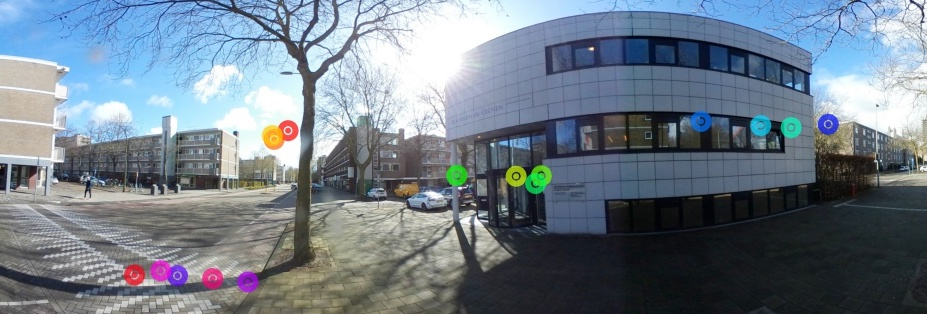
\includegraphics[width=\linewidth]{figures/2-met-video_sample.jpg}
\end{center}

\vfill

% In case of an internal project, remove External Supervisor or if you had two internal supervisors, change the header into 
%  & First Supervisor & Second Supervisor  \\
\begin{center}
\begin{tabular}{|l||lll|}
\hline
 & \textbf{Internal Supervisor}             & \textbf{1st External Supervisor}  & \textbf{2nd External Supervisor} \\   
\hline
\textbf{Title, Name} & Dr. Marcel Worring   & PhD, Jurriaan Schreuders          & Ir. Sander Buningh \\
\textbf{Affiliation} & UvA, FNWI, IvI       & Kexxu Robotics                    & BAM Infra \\ 
\textbf{Email}       & m.worring@uva.nl     & jschreuder@kexxu.com              & sander.buningh@bam.com \\
\hline
\end{tabular}
\end{center}


%% If you have a third supervisor use this table instead
%\begin{center}
%\begin{tabular}{|l||lll|}
%\hline
% & \textbf{External   Supervisor} & \textbf{External   Supervisor} & \textbf{3$^{\mathrm{rd}}$ supervisor} \\
% \hline
%\textbf{Title, Name} & Dr Maarten Marx& & \\
%\textbf{Affiliation} &UvA, FNWI, IvI & & \\ 
%\textbf{Email} & maartenmarx@uva.nl& &  .\\
%\hline
%\end{tabular}
%\end{center}

\bigskip

% logos
\begin{center}
\mbox{
    
\includegraphics[width=.2\paperwidth]{titlepage/logo-uva.png} 
    
\includegraphics[width=.2\paperwidth]{titlepage/ads.png}
}
\mbox{
    
\includegraphics[width=.2\paperwidth]{titlepage/kexxu.png}
    
\includegraphics[width=.2\paperwidth]{titlepage/bam.png}
}
\end{center}
\end{titlepage}

%
%\newpage
%
%\end{document}


\begin{abstract}
    As cycling is increasingly adopted as the future of sustainable mobility, governments are interested in making it safer. We use various senses during any traffic interaction, of which the visual is the most dominant. While eye-movement research in auto-motors is a mature field, the amount of research in cycling is relatively small. This research maps a single wearable eye-tracker to master footage using computer recognition, and evaluates both Scale Invariant Feature Transform (SIFT) and implementation of a Siamese Neural Network (SNN). Of both, SIFT obtained an accuracy of 52\% and the SNN an accuracy of 38.6\%. Both are not robust enough to build a reliable mapping but they can, however, establish a baseline for future research in this topic.
\end{abstract}

\maketitle


% \begin{tikzpicture}[remember picture,overlay,shift={(current page.north west)}]
% \node[anchor=north west,yshift=0.5cm,xshift=-0.2cm]{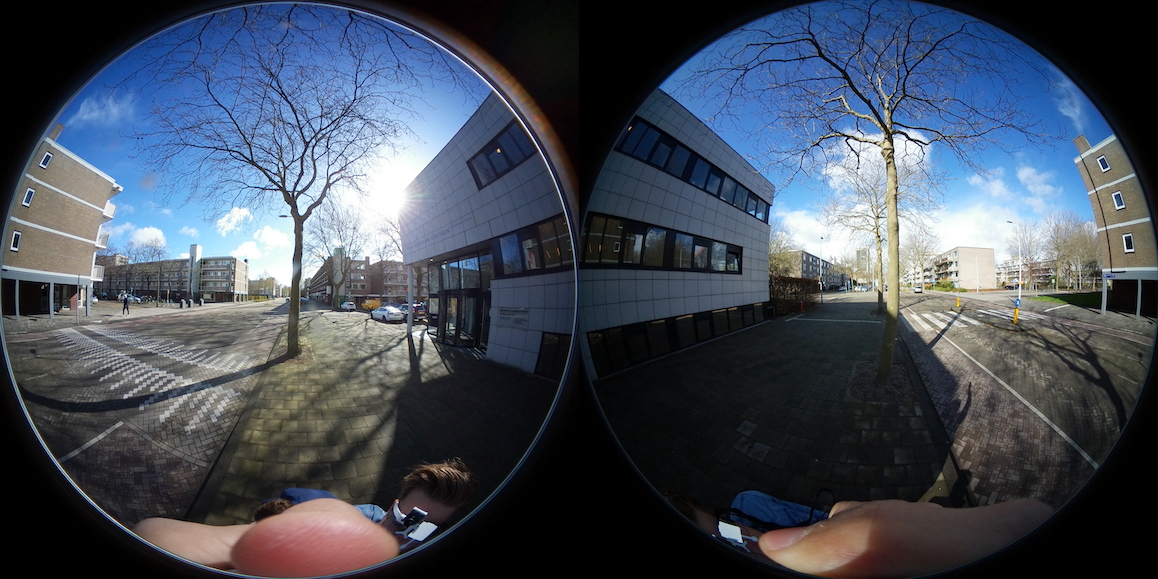
\includegraphics[width=\paperwidth, height=2.2cm]{figures/1 original.JPG}};
% \end{tikzpicture}


\begin{description}
     \item[Student] \href{mailto:ivo.de.geus@student.uva.nl}{Ivo Cornelis de Geus}
     \item[External Supervisor] \href{mailto:jschreuder@kexxu.com}{J. Schreuder, PhD}
     \item[External Supervisor] \href{mailto:sander.buningh@bam.com}{S. Buningh, Ir. }
     \item[Internal Supervisor] \href{mailto:m.worring@uva.nl}{Prof. Dr. M. Worring}
     \item[Video Footage] \href{https://youtube.com/playlist?list=PLzh4mA3kUCz2J9pJhzKEI88LiCYvB9BQk}{Playlist Link}
     \item[Thesis Repo] \href{https://github.com/idegeus/msc-ds-thesis}{idegeus/msc-ds-thesis}
     \item[Python Repo] \href{https://github.com/kexxu-robotics/video_heatmap}{kexxu-robotics/video\_heatmap}
\end{description} 
 
\section{Introduction}
    \subsection{Cycling \& Traffic Attention}
    Cycling is often touted as the future of personal mobility as it is a healthy, sustainable, cheap and fun mode of transport \cite{DeGeus2009, Hendriksen2010, St-Louis2014}. From a governments' perspective, citizens get significantly healthier, which is combined with a more efficient spatial urban character \cite{Nello-Deakin2019, Bruun1995}. With 68\% of the world population expected to live in urban areas by 2050, the United Nations deems Cycling such a good fit in its sustainability goals that it declared the third of June as the international cycling day \cite{UnitedNations2019, UnitedNations2018a, UnitedNations2018}. In aiming for these advantages, governments are increasingly looking for advice from countries with success stories in creating a cycling culture. Examples of these countries are the Netherlands, Denmark, and Germany \cite{Schepers2017}. An increasingly discussed measure to improve the "cycling climate" is a redistribution of urban space to prioritize one modality over the other \cite{Nello-Deakin2019, Gossling2020}. 
    
    Equally crucial as linked to the urban decisions is how transport is taking place and how it is perceived. When people navigate public spaces, they scan their surroundings mostly unconsciously to adapt and fit in in traffic \cite{HollanderJustinB.Sussman}. In a historical perspective, \citeauthor{VanGompel2007} refer to Du Laurens, a French anatomist and medical scientist in 1596: Du Laurens described the eyes as "windows of the mind". Indeed, it seems clear today that eye movements reveal the workings of the mind and the brain \cite{VanGompel2007}. \citeauthor{Just1980} name the the theory on eyes giving information about what the brain is processing the "eye-mind assumption" \cite{Just1980}. While this link does not directly guarantee processing by the brain, it is still strong and valuable indicator \cite{Berger2018}. 
    
    Since visual perception is the most crucial factor in navigation and perceptual errors make up 20\% of European road accidents, it makes sense to examine how we process this information \cite{ERSO2020, Reyes2008, VanGompel2007, Underwood2007}. It is an essential factor in obstacle avoidance, safe navigation, and risk perception and is, therefore, a large part of the required workload to participate in traffic \cite{Lehtonen2014, Werneke2012}. Using eye-tracking in traffic studies is therefore not a new idea: both for in car-driving and walking, eye movements are studied extensively to evaluate driver awareness \cite{Stapel2020}, intersection design \cite{Werneke2012, Crundall2011}, location, colors, fonts of signage \cite{HollanderJustinB.Sussman}, and the impact of information in advanced driver assistant systems \cite{Reyes2008, Kohl2020, OsbeckEmelieAkerman2010}, to name but a few.  While \citeauthor{OsbeckEmelieAkerman2010} argues eye-tracking is not sensitive enough to be used for workload measuring, it has sometimes been used to determine behavior, comfort, and workload in traffic situations \cite{OsbeckEmelieAkerman2010, Mantuano2017a, Berger2018, Cegovnik2018c, Bongiorno2017a}. The amount of research in the visual behavior in cycling (as an urban transport) used to be limited and has seen an uptake in recent years \cite{Lehtonen2016, Vries2017, Mantuano2017a, Trefzger2018, Kovacsova2018, Rupi2019, HollanderJustinB.Sussman}. This field still holds much potential for further research, as \citeauthor{ERSO2020} claims that in the period 2010 to 2020, cycling was the only modality not decreasing in fatalities. Cycling is strongly dependent on visual perception in more ways than one, as several studies have shown that even a perceived lack of safety can be a deterrent to cycling \cite{Fishman2012}. For this reason, it makes sense to pay close attention to where cyclists are looking and how they are paying attention. 
    
    \subsection{Wearable Eye-Trackers} %.
    Running an eye-tracking experiment on the topic of traffic is usually done in a controlled environment at a desk with a fixed eye-tracker such as in \cite{Velichkovsky2003, Werneke2012, Reyes2008}. While this has many advantages, such as internal validity, reliability, and ethical advances, a possible lack of realism and ecological validity of a desk-mounted eye-tracker is a disadvantage, primarily to behavior research in real-life \cite{Vansteenkiste2015, Zeuwts2016}. 
    
    For this purpose, several different wearable eye-trackers have been developed, such as the versions used in \cite{Mantuano2017a, Zeuwts2016, Rupi2019, Gruden2021, Trefzger2018}. This type of eye-tracker captures the participant's perspective, with the relative eye movement projected on top. While fixed eye-trackers can generate an aggregated map of Areas of Interest (AOI) as the scene is always the same, the different head movements and behavior of different participants make this more complicated as there is no single map to project on.
    
    \subsection{Relative \& Absolute Coordinates}
    With fixed desktop eye-trackers, views and observations are directly mapped to an absolute coordinate system in, usually, the screen. The resulting footage is called a map of Areas of Interest (AOI). A wearable eye-tracker generates gaze coordinates relative to the wearable's frontal camera, and not to the coordinates of the static objects in the environment. In previous studies, this has been resolved by analyzing the scene frame-by-frame and fixation-by-fixation, described by \citeauthor{Duchowski2007} as "rather tedious but surprisingly effective", and has been used successfully by several other researchers \cite{Duchowski2007, Mantuano2017a, Vansteenkiste2015}. These types of analysis are sometimes further developed into gaze plots to see the order of scanning through the environment, e.g., whether users first look right and then left or the other way around as done in \cite{Gruden2021}. 
    
    \begin{figure}
        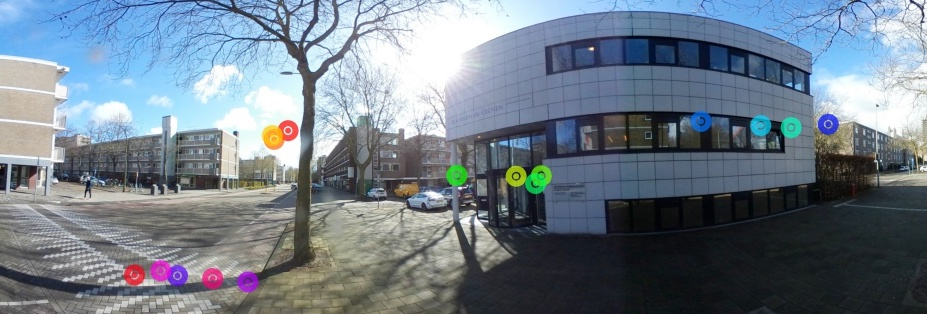
\includegraphics[width=\linewidth]{figures/2-met-video_sample.jpg}
        \caption{Generated mock-up of the desired result of merged eye-tracking data of 16 participants, four groups with clear different behavior. See an animated example in the playlist at the start of this paper or \href{https://youtube.com/playlist?list=PLzh4mA3kUCz2J9pJhzKEI88LiCYvB9BQk}{here}.}
        \label{fig:mapped-example}
    \end{figure}
    
    As these methods are highly qualitative with an extensive workload for researchers, increasing the number of participants and gaining extra information directly increases the workload of extracting information, which could explain why the mentioned studies use between 5 and 20 participants \cite{Rupi2019, Gruden2021, Trefzger2018}. Gaining this information about differences might be helpful to provide insight into where multiple groups of participants are looking and possibly making distinctions between groups. It could be interesting, for example, to create a distinction between the viewing patterns or amount of tunnel vision of different age groups or using an e-bike or a regular city bicycle. While these kinds of distinctions can currently be made with wearable eye-trackers, their potential in decreasing researcher workload is considerable, especially if these conclusions can be drawn by an algorithm instead of manually assigning values. 
    
    As far as we could find, a combination of the different fields of wearable eye-tracking and panoramic imagery mapping does not yet exist. While existing software\footnotemark does enable multiple eye-trackers to be mapped to a similar point-based on image stills extracted from the frontal scene-cam, this is neither automated nor applicable for a longer duration, for example, tracking a full cycling itinerary or a traffic intersection with multiple participants. The mentioned existing eye-tracking studies contributed in the fields of, to name two, intersection design \cite{Rupi2019, Werneke2012, Kovacsova2018, Mantuano2017a} and perception of danger in natural conditions \cite{Underwood2007, Liu2011, Lehtonen2016, VanGompel2007}. These fields should be able extract more information quickly when the process of adding more participants and aggregating these data is streamlined. 
    
    \footnotetext{For example, the toolkit for the \href{https://www.tobiipro.com/learn-and-support/learn/steps-in-an-eye-tracking-study/data/manual-and-assisted-mapping/}{TobiiPro} wearable, which is proprietary software. }
        
    The absence of existing solutions leads us to the current project. In this research, a method is created to map a wearable eye-tracker on one single master image using a computer vision feature detection system. The relative gaze coordinates of wearable eye-trackers are mapped onto one single master track. To determine where specific points are located on the "base image", we propose the usage of a one-shot image recognition architecture, in this case, a Siamese Neural Network (SNN), which we will introduce in \autoref{sec:relatedworks}. 
    
    To summarize, this paper aims to bring contribution to the following topics. 
    
    \begin{itemize}
        \item Expanding on the usefulness of eye-tracking in traffic interactions.
        \item Enabling a new research method by increasing the viable amount of participants in a wearable eye-tracking study.
        \item Evaluating the usefulness and accuracy of computer vision in mapping two images from streetscape together. 
    \end{itemize}
    
    \subsection{Research Questions}
        This research is divided into three research questions to establish concrete and measurable goals. RQ1 aims at establishing a baseline using a traditional computer vision algorithm. We will elaborate further on this method based on feature extraction, such as corner- and contrast-detection, in \autoref{sec:traditionalcomputervision}. We introduce this method to set a baseline for comparing the second method. For RQ2, we will introduce a SNN which takes a different approach, as explained in \autoref{sec:snn}. For RQ3, a video will be generated based on captured footage using the best functioning model. 
    
        \begin{itemize}
            \item[RQ1] How well can SIFT detect fragment location? 
            \item[RQ2] How well can a SNN detect fragment location?
            \item[RQ3] How can an aggregated AOI panoramic map of several wearable eye-trackers be created?
        \end{itemize}

\section{Related Works}\label{sec:relatedworks}
        
    \subsection{One-shot Image Recognition}
        Mapping several different images onto one master image without having the ability to train based on classical labeled examples (supervised learning) can be considered a case of one-shot image recognition. This problem is defined as being able to learn information about an object from one or only a few training samples or images \cite{WikipediaOneShotLearning2021}. It is a problem that humans are shown to be good at in early development stages due to the ability to synthesize and learn new object classes from existing information about previously learned classes. This usage of previously learned knowledge is the key motivation for one-shot learning techniques, where systems can, as humans, use prior knowledge to classify new objects \cite{Fei-Fei2003, Fei-Fei2006}. The basis for this topic was laid by  \citeauthor{Fei-Fei2003} \cite{Fei-Fei2003}. In this paper, a variational Bayesian framework for one-shot image classification was created based on the idea that previously learned classes could help forecast future ones. Candidate architectures that are based on this principle might provide a solution direction. Computer vision models for one-shot learning are divided into either feature learning or metric learning. In this project, we will build an implementation for both these categories. We will use the SIFT algorithm for the first, and the Siamese Neural Network for the second. 
        
    \subsection{Traditional Computer Vision}
        \label{sec:traditionalcomputervision}
        Scale-Invariant Feature Transform (SIFT) works by first generating reference keypoints from a set of images, to which a new image is then compared  \cite{Low2004, Wan2013}. The patent on this algorithm expired late 2020 and it is now incorporated in the OpenCV library \cite{OpenCV2020}. SIFT works by adding Gaussian convolutions over differently oriented- and scaled grey-scale versions of an image, and comparing the Euclidean distance (\lstinline{cv.NORM_L2}) between detected keypoint vectors in those convolutions. By comparing these vectors to the new image, similarity between images can be identified. SIFT is selected because its generated keypoints are robust against several types of clutter, including different scaling, orientation, brightness, and partly to affine distortion. 
        
        While SIFT can locate a fragment inside a global image, giving a definite position directly, we decided to evaluate both systems by the same method, opting to extract a similarity score instead. We believe this made the comparison between this method and the following method clearer. 
        
    \subsection{Siamese Neural Networks}\label{sec:snn}
        Another approach that uses the same core principle are Siamese Neural Networks (SNNs), which were first introduced by \citeauthor{Bromley1993} to solve the signature matching problem. This section is partly based on the explanation from \citeauthor{Koch2015} in \cite{Koch2015}. The core problem a SNN intends to solve is generating a robust representation in a multi-dimensional space, optimizing for a low distance between same-class objects and a high distance between different objects. Training such a network is typically achieved by creating two image augmentations, subject to certain conditions to avoid collapsing solutions \cite{Chen2020a}. 
        
        \begin{figure}
            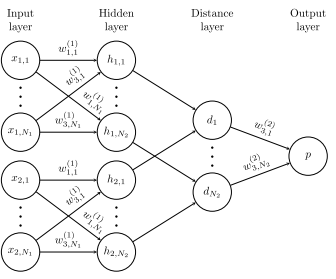
\includegraphics[width=\linewidth]{figures/1-rl-snn.png}
            \caption{From \citeauthor{Koch2015} \cite{Koch2015}: Simple 2-hidden-layer Siamese Network for binary classification with logistic prediction $p$. Top and bottom networks are twins with shared weight matrices.}
            \label{fig:1-rl-snn}
        \end{figure}
        
        \begin{figure}
            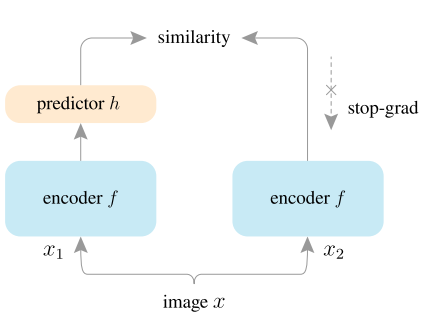
\includegraphics[width=\linewidth]{figures/1-rl-chen2020fig1.png}
            \caption{SimSiam Architecture with a single predictor $h$ and stop-grad on the second twin, from \citeauthor{Chen2020a} \cite{Chen2020a}, page 1}
            \label{fig:1-rl-chen2020fig1}
        \end{figure}
        
        While many SNNs have been proposed and tried, a more typical SNN consists of two twin networks accepting different inputs, joined by an energy function at the top, see Figure~\ref{fig:1-rl-snn}. As visible, in this example, both networks use the same weight sets, which ensures both the consistency and symmetry of predictions, as both sides of the network will output the same function. 
        
        The architecture used in this project was introduced by \citeauthor{Chen2020a}, called Simple Siamese Representation, short SimSiam. In their paper, \citeauthor{Chen2020a} explore the effects of deliberately introducing a stop-gradient on the second "twin" of the SNN, which showed its effectiveness \cite{Chen2020a}. This version of a SNN showed an accuracy of 68.1\% on the ImageNet-dataset. The rest of this paragraph will briefly give an oversight of the structure of the used SNN as explained in \cite{Chen2020a} and \autoref{fig:1-rl-chen2020fig1}. The network takes in two random augmentations $x_1$ and $x_2$ from image $x$. The two images are processed by an encoder network $f$, which consists of a backbone (in this case, ResNet) and a projection Multilayer Perceptron (MLP). The encoder $f$ shares weights between the two views, as shown in \autoref{fig:1-rl-chen2020fig1}. Prediction head $h$ transforms the output of $f_1$ and matches it to the other unprocessed view $f_2$. In training, their cost function is defined as the negative cosine similarity between the two views. See for a detailed explanation \cite{Chen2020a}.   
        % Lots more explanation about neural networks and the specific type chosen in this paper to come here, using \cite{Roy2019} and \cite{Koch2015} as general sources and \cite{Chen2020}
    
\section{Methodology}\label{sec:methodology}
    The initial concept of creating a heat-map takes one panoramic master image and using video footage from the wearable eye-tracker to map on this image as shown in \href{https://www.youtube.com/playlist?list=PLzh4mA3kUCz2J9pJhzKEI88LiCYvB9BQk}{the example in this link\footnotemark}. A panoramic image mainly exists in two forms: dual fish-eye, which is the raw output of two lenses on the camera, and equirectangular, which is a stitched and rectangular projection of the source. See an example of this behavior in \autoref{fig:2-met-fisheye-stitched} in the appendix on page \pageref{fig:2-met-fisheye-stitched}. To compare the eye-tracker to this image, we will use the equirectangular projection. 
    \footnotetext{See \href{https://www.youtube.com/playlist?list=PLzh4mA3kUCz2J9pJhzKEI88LiCYvB9BQk}{youtube.com/playlist?list=PLzh4mA3kUCz2J9pJhzKEI88LiCYvB9BQk}.}
    
    In this stage, the mapping will only work when the participant wearing the eye-tracker is standing at the same point as the master image is created. As the eye-tracker returns a JSON file with the estimated coordinates of the tracked pupil per frame, this can be mapped on the master image when its location is determined, see \autoref{2-met-movinggrid}. To compare and evaluate the different methods which will be tried, the footage from the eye-tracker will have to be hand-labeled to establish ground truth. Every frame is compared to an extracted grid of footage of the panoramic camera, from which the most similar will be saved. The performance of both methods will be measured in the distance between the predicted position to the target (hand-labeled) position in pixels, where some margin can be taken in labeling a guess as correct as the base frames will not always be a perfect fit.
    
    The workflow and procedure in this experiment are therefore as follows: 
    
    \begin{enumerate}
        \item Grab panoramic image or video as master-track. 
        \item Unroll, stabilize, and crop panoramic footage.
        \item Collect eye-tracker footage and data.
        \item Hand-label correct location of eye-tracker footage.
        \item In case of SNN: Divide panoramic footage in excerpts to compare to the eye-tracker footage.
        \item Compare the accuracy of different mapping methods.
    \end{enumerate}
    
    \subsection{Computer vision}
    Regarding the computer vision architectures, SIFT was selected as a baseline, using the existing open implementation by OpenCV2 \cite{OpenCV2020, OpenCV2020a}. For the SNN, an open-source implementation on Github with pre-trained weights was found and used\footnotemark.
    \footnotetext{See \url{https://github.com/taoyang1122/pytorch-SimSiam} for this implementation}

    \begin{figure}
        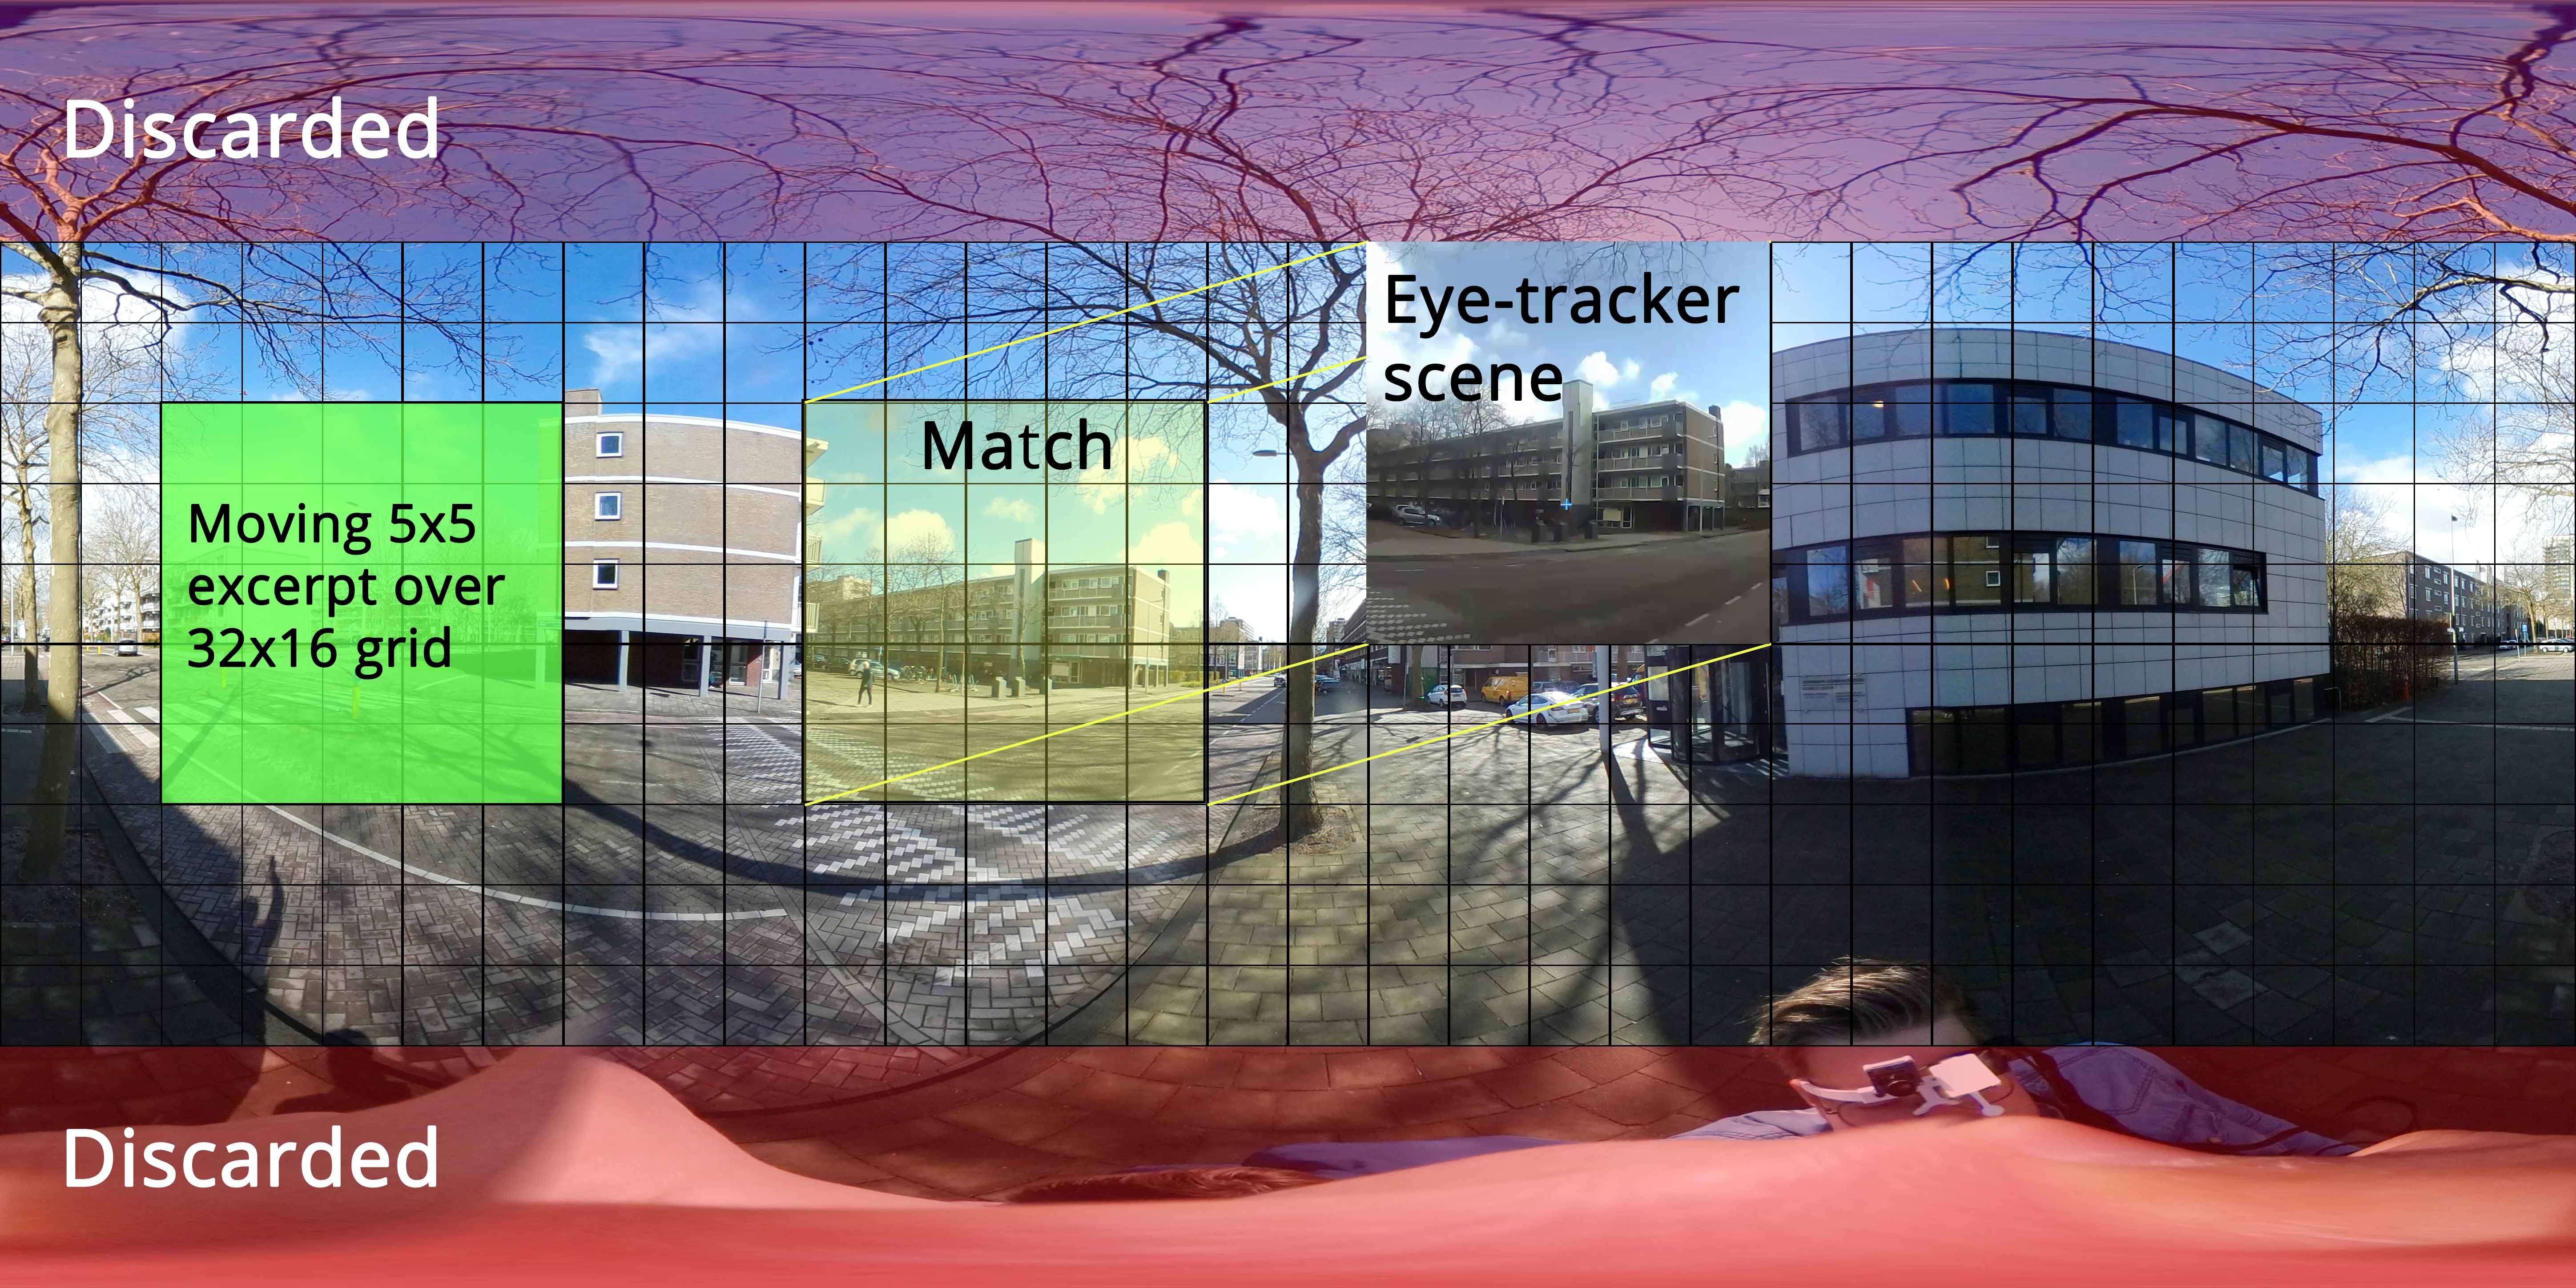
\includegraphics[width=\linewidth]{figures/2-met-movinggrid.jpg}
        \caption{Visual explanation of comparison check.}
        \label{2-met-movinggrid}
    \end{figure}
    
\section{Experiments}
    \subsection{Hardware Used}
    The eye-tracker used in this project is a beta-version of OpenEye, a prototype wearable eye-tracker made by Kexxu, see \autoref{3-exp-openeye} on page \pageref{3-exp-openeye}. This version uses a pre-trained neural network on a portable Raspberry PI to interpret pupil location in real-time\footnotemark. While it is normal for eye-trackers to incorporate and distinguish between saccades and fixations \cite{VanGompel2007}, this eye-tracker was not equipped with this capability. A 3D-printed wearable frame with one pupil-facing camera and one scene-facing camera are combined directly in one combined MP4 video file (1280x720, 14fps) and a JSON file with relative projected focus positions. Every frame was center-cropped to 720x720 pixels to be used in the different image recognition methods. 
    \footnotetext{See \url{https://kexxu.com} for more details about the eye-tracker used.} 
        
    \begin{figure}
        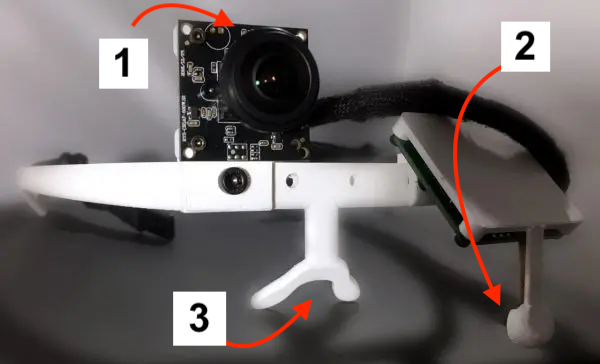
\includegraphics[width=\linewidth]{figures/3-exp-openeye.png}
        \caption{OpenEye wearable consisting of (1) a scene-camera, (2) a left-eye facing camera and (3) the nose-bridge of the 3D-printed frame. }
        \label{3-exp-openeye}
    \end{figure}

    The footage grabbed for this Proof of Concept was 18 seconds of footage, a total of 245 frames, at a single location with an accurate embedded eye-tracking registration. The location for this initial test was in Amsterdam, near the office of Kexxu at the A. J. Ernststraat. This is an urban location with plenty of possible features to be extracted. 
    
    Another piece of footage using both the panoramic camera and the eye-tracker was grabbed near the north, near Alkmaar. This footage was discarded as it was of low quality with the eye-tracker crashing mid-way due to a battery failure. Instead, the project was carried out using the footage recorded in Amsterdam.
    
    The camera used for grabbing the master footage, in this case, a panoramic picture, is the Samsung Gear 360 II, which can grab both panoramic images and videos\footnotemark. \footnotetext{For specifications, see \url{https://www.samsung.com/global/galaxy/gear-360/}.} The footage unrolled is of a resolution of 5792×2896. 
        
    \subsection{Software Used}
    A Flask-React service was built to hand-label the correct position of each frame on the master footage and to validate the accuracy of several methods\footnotemark. The footage generated by the panoramic camera was pre-processed using Cyberlink ActionDirector, which offered the conversion to an equirectangular plane. Further processing and analysis is done in Jupyter Notebooks in a Conda-environment. 
    \footnotetext{See the GitHub repository for this service.}

\section{Results}
    This section on results will give results ordered per research question and immediately discuss it. In the next section, Conclusions, we will summarize and close off. 

    \subsection{RQ1: SIFT Performance}
        \subsubsection{Results}
        We used Scale-Invariant Feature Transform to establish a baseline to evaluate this classic computer vision architecture and compare the SNN effectively. Existing sample code fragments provided by the software package OpenCV were used to establish this section \cite{OpenCV2020, OpenCV2020a}. In evaluating the accuracy, we used the same technique as in the Siamese Neural Network, in comparing fragment-wise (as shown in \autoref{2-met-movinggrid}) and selecting the image with the highest amount of matched keypoints as suggested by \cite{OpenCV2020}. 
        
        All frames were compared using SIFT to the square extracts from the panoramic camera, where an accuracy within two frames from the target point of \textbf{52.03\%} was achieved. The locations where this algorithm fails to identify accurately seem to be darker images and images, including fewer overall keypoints. In \autoref{fig:sift-sample}, the first image is correctly identified and the second and third incorrectly. For a comparison of more frames, see \autoref{fig:4-res-comparisons} on page~\ref{fig:4-res-comparisons}. 
        
        \begin{figure}
            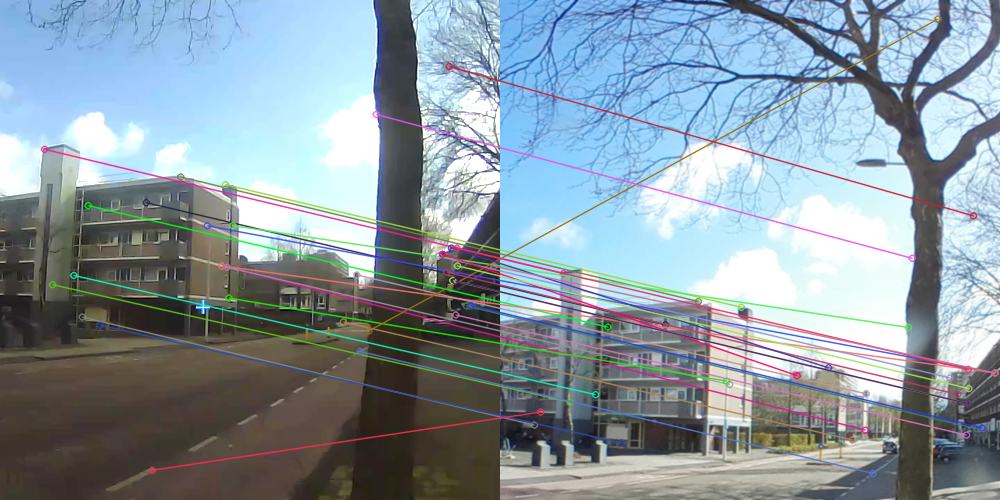
\includegraphics[width=\linewidth]{figures/4-sift1-048.png}
            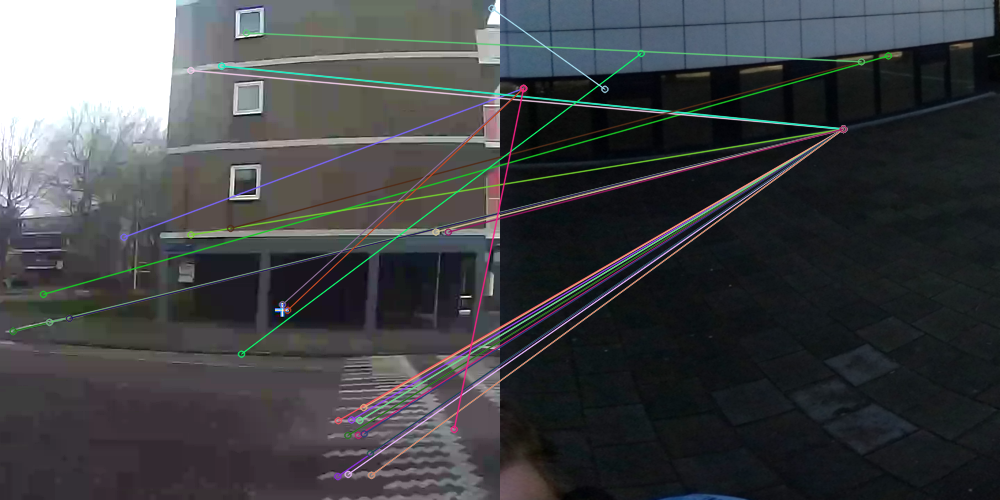
\includegraphics[width=\linewidth]{figures/4-sift2-117.png}
            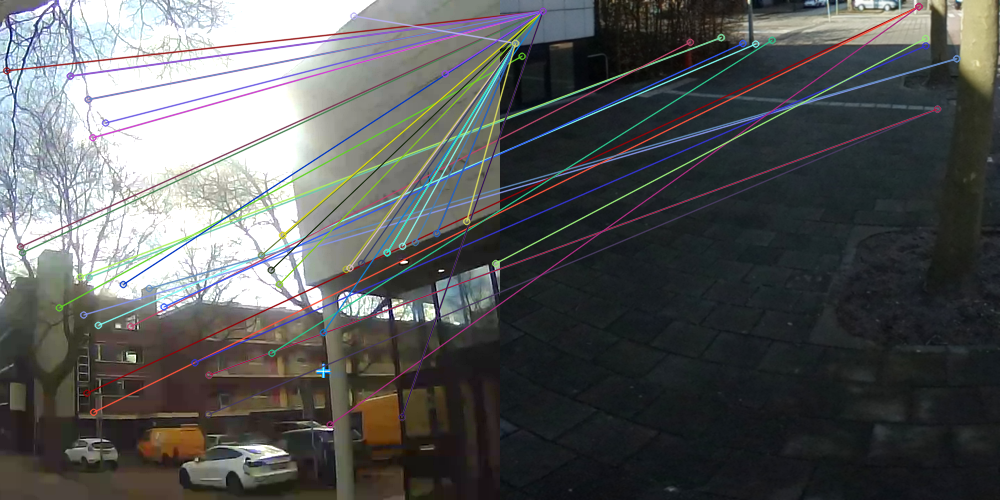
\includegraphics[width=\linewidth]{figures/4-sift3-143.png}
            \caption{Three samples generated by SIFT: Left is the original eye-tracker scene camera, right is the estimated scene. } 
            \label{fig:sift-sample}
        \end{figure} 
    
        \subsubsection{Discussion}
        In the current setup, this method performed as expected, with some exceptions, such as the different affine transformations of the two different images and the difference in image quality. While SIFT is known to be resistant to scale and orientation, its ability to cope with different transformations as done by the transforming software of a panoramic camera is limited. This difference is evident when seeing the whole image, such as in \autoref{2-met-movinggrid}. One solution could be to, instead of mapping the panoramic footage on an equirectangular plane, mapping it on a projection based on the faces of a cube as done in \cite{Davidson2020}. This alternative projection could reduce distortion and allow for better performance of this algorithm. 
        
        Another reason the algorithm fails to map some points correctly are darker images or images with less possible assignable keypoints in the master image. Darker spots in the images, such as the hard shadows generated by the low sun in the spring, can explain the tendency to be mapped to those points. A lack of features might be more difficult to resolve using SIFT, especially since SIFT works in grey-scale \cite{Low2004}. An upside here is that these points of failure are usually sequentially between correctly mapped images, so smoothing could be applied to detect outlier image detection. One example of this method could be as follows: the eye-tracker captures at 14 frames per second, which limits the physical movement between frames. If one frame is on the other side of the map, surrounded by 2 frames on both sides on the other side of the map, this could be flagged as incorrect, and be interpolated between the two other frames. 
        
        One last quick-win with SIFT could be to detect the overall angle between keypoints. If a part of keypoint vectors angle up or down as seen in the first image in \autoref{fig:sift-sample}, this could easily be corrected to a different vertical position, correcting the actual height. In a sense, this is caused by the deviating practice used in SIFT, as it can normally pinpoint an exact location instead of generating a similarity score. 
    
    \subsection{RQ2: Siamese Network Performance}
        \subsubsection{Results}
        The SNN used has been pre-trained using the resources in the GitHub repository, which is the setup we will use here too. All 245 frames of the eye-tracker and the grid of 32x6 extracts of the base image were run through the SNN. These images were compared using the negative cosine similarity metric as proposed in the original paper. The pre-training was done using batches of 432 with a learning rate of 0.1 \cite{Chen2020a}.
        
        Using this method, accuracy of estimation within 2 frames around the center track was created of \textbf{38.6\%}, see some examples and their scores (expressed as a fraction of a deviation of 181px, 1 frame) in \autoref{fig:4-res-comparisons} on page \pageref{fig:4-res-comparisons}.
    
        \subsubsection{Discussion}
        This early version of the SNN shows potential but performs worse than the baseline set by the SIFT algorithm. However, its potential is there, especially considering it is only trained based on object recognition from ImageNet. When implementing a version in follow-up research, focusing more on making streetscape comparisons could increase the accuracy, which can be trained using datasets such as \cite{Cordts2016TheUnderstanding}. One other way of improving this neural network is by incorporating an algorithm correcting for the distorted lines in the equirectangular as done in \cite{Deng2017}. We believe that making these changes in a second iteration of this project could improve the accuracy by a big margin. 
        
        As visible in the graph in \autoref{fig:4-res-deviation-distribution}, a big part is within the two frames of deviation from the target position. This deviation is the part that can be explained as similar features exist both in the source and target frame. The parts determined beyond the first spike are created by noise and are inaccurate. These are, for example, the third, fourth, and fifth images in the examples in \autoref{fig:4-res-comparisons}.
        
    \begin{figure}
        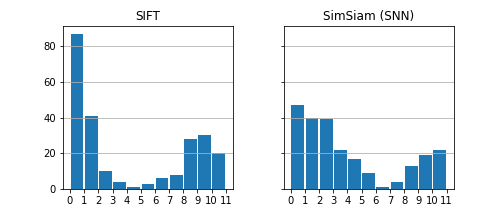
\includegraphics[width=\linewidth]{figures/4-res-deviation-distribution.png}
        \caption{Distribution of distance of estimated fragments to the true coordinates. Lower is better.}
        \label{fig:4-res-deviation-distribution}
    \end{figure} 
    
    \subsection{RQ3: Creation of panoramic AoI-Map}\label{sec:res-RQ3}
        \subsubsection{Results}
        The results of both methods are assembled into a video as proposed in \autoref{sec:methodology}, which is available \href{https://www.youtube.com/playlist?list=PLzh4mA3kUCz2J9pJhzKEI88LiCYvB9BQk}{on YouTube} (see link in \autoref{sec:methodology}). See an example frame from one of the videos in \autoref{fig:4-res-mapping-example}.  
        
        \begin{figure}
            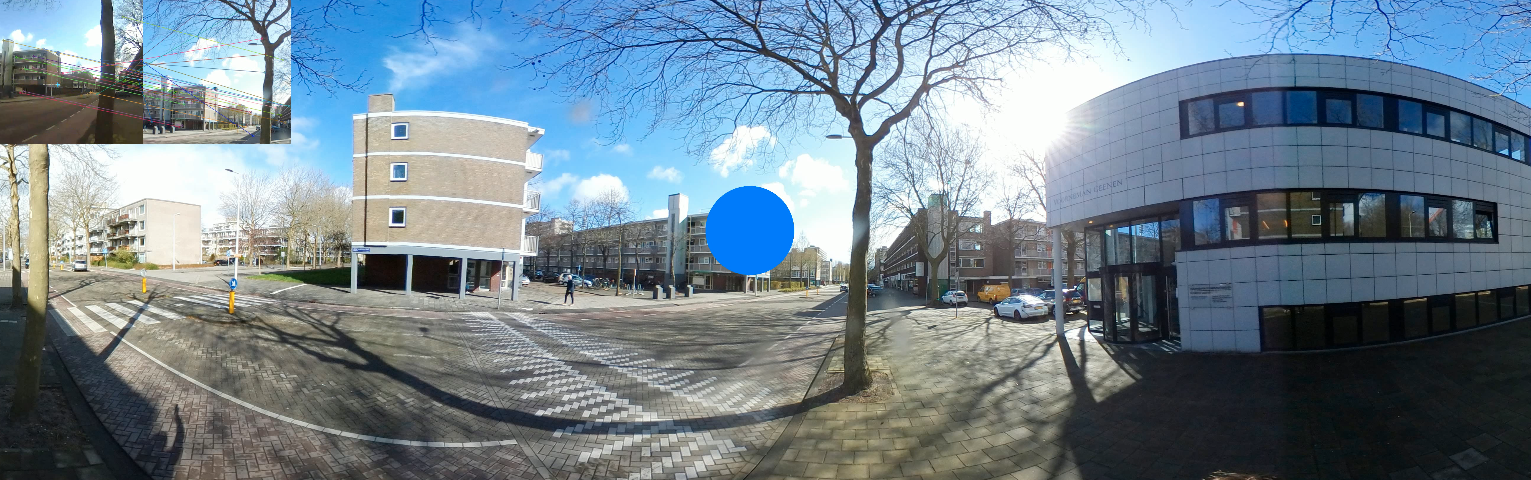
\includegraphics[width=\linewidth]{figures/4-res-mapping-example.png}
            \caption{Example frame from the generated video, with a blue indicator positioned around the current gaze position.}
            \label{fig:4-res-mapping-example}
        \end{figure} 
        
        \subsubsection{Discussion}
        In both videos, the reliability of the used method is clearly visible, as the indicator of the current gaze position is not consistently accurate. In future works, a number of factors could help to improve accuracy and generate a consistent video, in summary: 
        \begin{itemize}
            \item Film master footage on a day without harsh light (overcast clouds).
            \item Unroll and pre-process footage with minimal distortion, unrolling on the faces of a cube. 
            \item Smooth out fast movements and collapsing of algorithms by interpolating incorrect frame locations. 
            \item Further optimize SIFT extraction by using exact mapping instead of similarity. 
            \item Add further training to SNN using augmentations of streetscapes as source images. 
            \item Combine results from SIFT and SNN to complement their strengths (feature-rich areas vs color-distinctions). 
        \end{itemize}
        
        When expanding this trial into the final goal of employing multiple eye-trackers on a shared itinerary, several other practical factors in experimental approaches have to be considered. For one, both the master track and the individual itineraries should be recorded separately, with spatial location data available for each recorded frame. Using this, the correct master image that is closest can be determined. Another factor to consider is that all run itineraries should be run in relatively quick succession, as imagery and landscape can change, which can cause obstacles in the two different algorithms detecting the correct positions. 

\section{Conclusion}
    In this project, we have aimed to enable a new research method by gaining aggregate summaries of gaze- and eye-tracking. The scene detection by feature extraction in this first version appears more potent than the Siamese Neural Network. This difference can be due to the SNN's nature, as only the standard pre-trained version was used in this project, and no changes have been made to improve the base accuracy. The SIFT algorithm used showed an accuracy of 52\% around the focus point. We hypothesize this accuracy should be enough to interpolate and make adjustments for the wrongly detected fragments using the sequential nature of the used video. While the used Siamese Neural Network shows an accuracy of 68.1\% in the original paper \cite{Chen2020a} and thereby created high expectations, we reached an accuracy of 38.6\% within a margin of about 362 pixels centering the focus point. There are a number of ways which can help increase the accuracy, both in experimental approach and algorithm improvements, as discussed in \autoref{sec:res-RQ3}. We hope that a follow-up project can improve this accuracy and enable the research method as proposed in this project. 
     
\section{Acknowledgements}
    Thank you to Jurriaan Schreuder for providing resources and guidance for this thesis, and inspirational space to work with colleagues. I learned a lot while working on this project, for which I am thankful. A special thanks to the people I have discussed this idea with and who have provided me with guidance, such as Sander Buningh and Marco te Brömmelstroet. 
    
    Marco brought me in contact with Sander, with whom I discussed mobility and innovation in this field, to be referred to Jurriaan. Together we came up with this concrete subject, for which I am very thankful. We had a great field-day at the Velodrome, organised by BAM Infra, during which i got to meet everyone in "real life". Lastly, thank you to my supervisor at the University of Amsterdam: Marcel Worring for his quick and extensive feedback and supervision during this project. 

\begin{landscape}
    \begin{figure}
        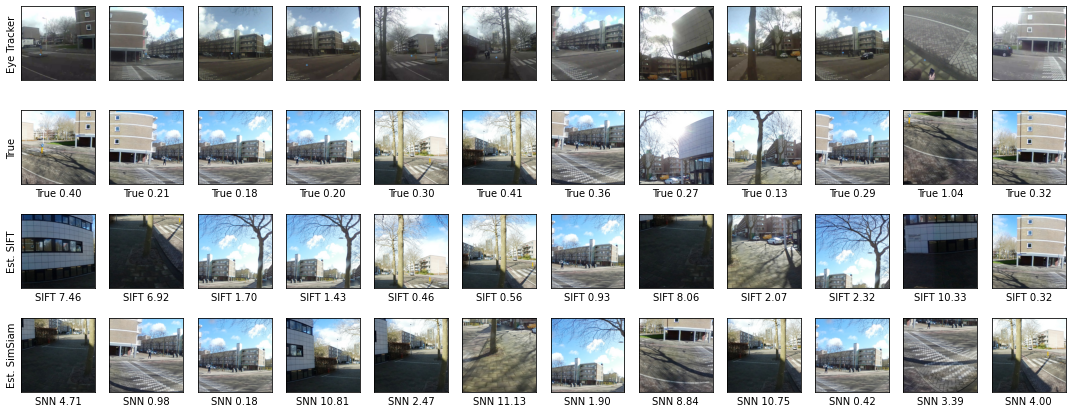
\includegraphics[width=\linewidth]{figures/4-res-comparisons.png}
        \caption{Twelve sampled frames. Score (lower is better) is amount of \emph{excerpts} of deviation from the defined ground truth.}
        \label{fig:4-res-comparisons}
    \end{figure} 
\end{landscape}

% your refs
\section{References}
\printbibliography[heading=none]

\appendix
\section{Panoramic projections}
\begin{figure}[h]
    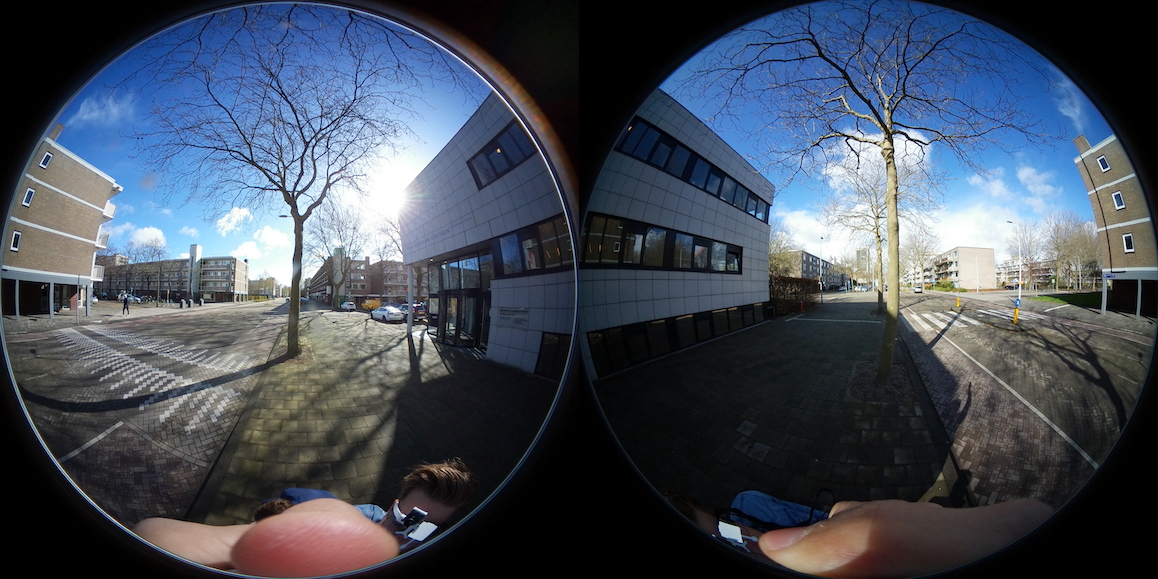
\includegraphics[width=\linewidth]{figures/2-met-fisheye.JPG}
    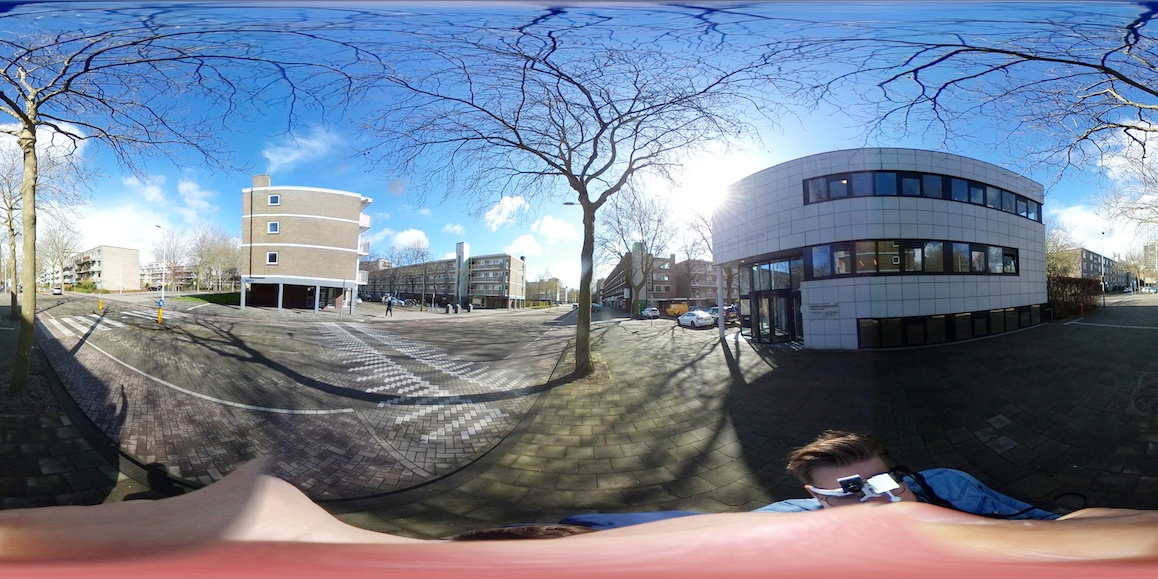
\includegraphics[width=\linewidth]{figures/2-met-stitched.JPG}
    \caption{Behavior of a fish-eye capture and the equirectangular flat render.}
    \label{fig:2-met-fisheye-stitched}
\end{figure}

\end{document}